\section{Architecture}
\label{sec_arch}


\subsection{System Architecture}

\begin{figure}[t]
\centering
   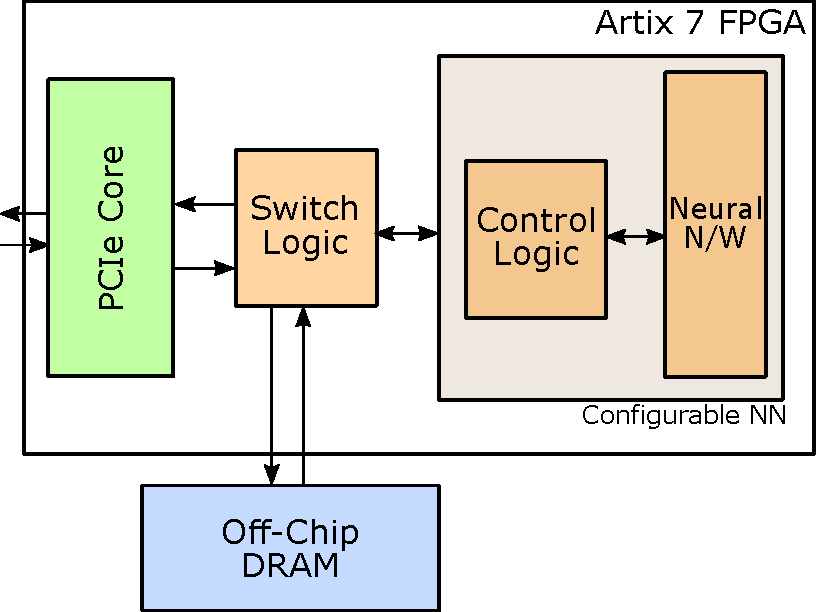
\includegraphics[height=0.7\columnwidth]{Figures/systemarch.pdf}
   \caption{Architecture of the proposed FPGA based neural network evaluation platform}
   \label{fig:sysArch}
\end{figure}

The system-level architecature of proposed FPGA based neural network accelerator platoform is as shown in Fig.~\ref{fig:sysArch}.
It is implemented on a off the shelf vendor supported FPGA development board (Xilinx~AC701).
The FPGA communicates with a standard host computer through PCIexpress interface to send data samples and to receive the processed output.
For the chosen platform, this communication link provides up to 2 GB/s communication bandwidth.
The FPGA board also has an on-board DDR3 memory for temporary data storage.

We use our previously developed open-source FPGA switch IP core for interfacing the PCIe core, DRAM memory controller and the neural network accelerator~\cite{blanked}.
Through software control, the training data, weights and test data can be either stored in the DRAM or directly injected to the neural network.
For the PNN implementation, the data is directly injected to the neural network since the modified architecture is capable of storing the entire training data in the FPGA itself.
The interfacing logic (PCIe and DRAM) and the switch logic remains the same irrespective of the neural network implemented on the FPGA platform.

The control logic block shown in Fig.~\ref{fig:sysArch} is specific to the target neural network architecture.
It is responsible for generating the global control signals, which controls the storage of weights (training data in case of PNN) inside the appropriate neurons.
It also acts as the input later for PNN where it accepts data from the switch and converts it into the specific format required by the neural network.
The neural network block implements all the remaining layers of the neural network, such as pattern, summation and output laters of PNN.
The number of classes in the pattern layer and the number of neurons in each class can be configured at design time.
The automation tool automatically generates the HDL code corresponding to the chosen parameters.

\subsection{Neuron}
\begin{figure}[t]
\centering
   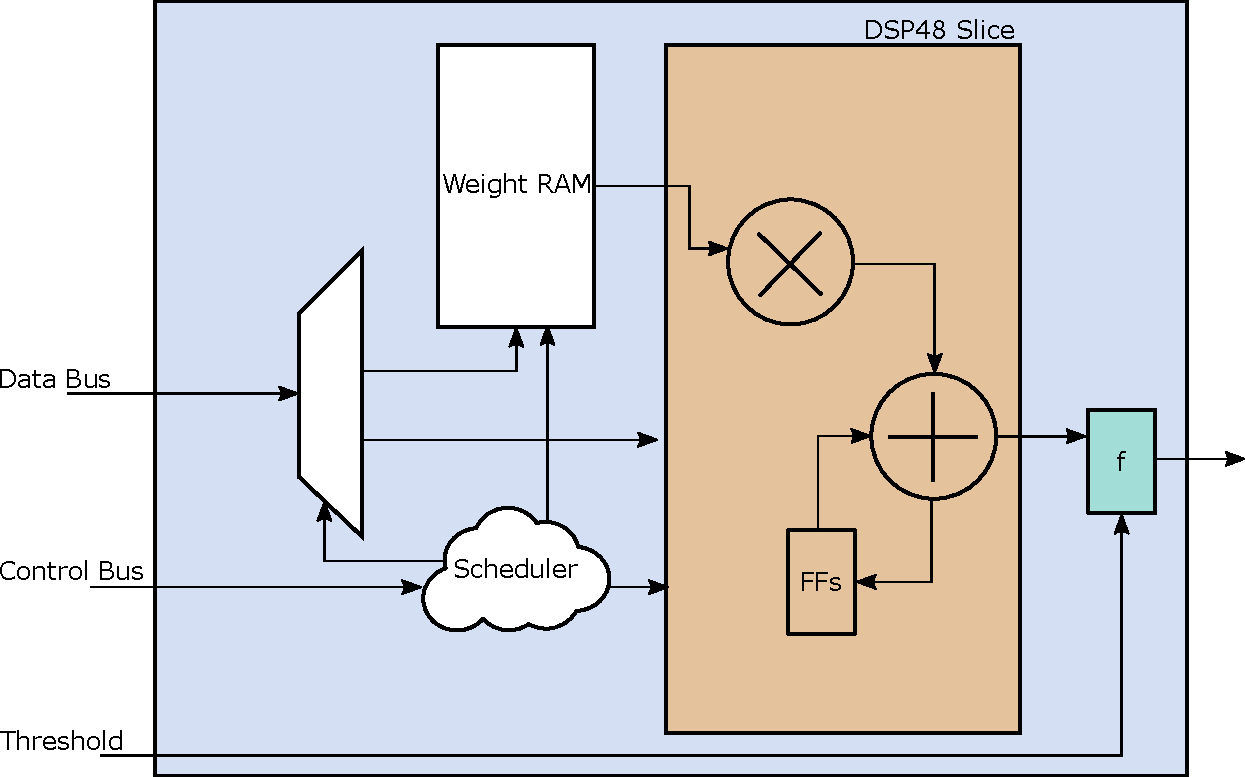
\includegraphics[height=0.5\columnwidth]{Figures/neuron.pdf}
   \caption{Architecture of a single Neuron using Xilinx DSP48 slice}
   \label{fig:neuron}
\end{figure}
The architecture of a single neuron used in the PNN pattern layer is depicted in Fig.~\ref{fig:neuron}.


\begin{enumerate}
\item Approximation of gaussian using threshold
\item Fixed point approximation
\item Advantages and limitations
\item Training and testing





\begin{figure}[t]
\centering
   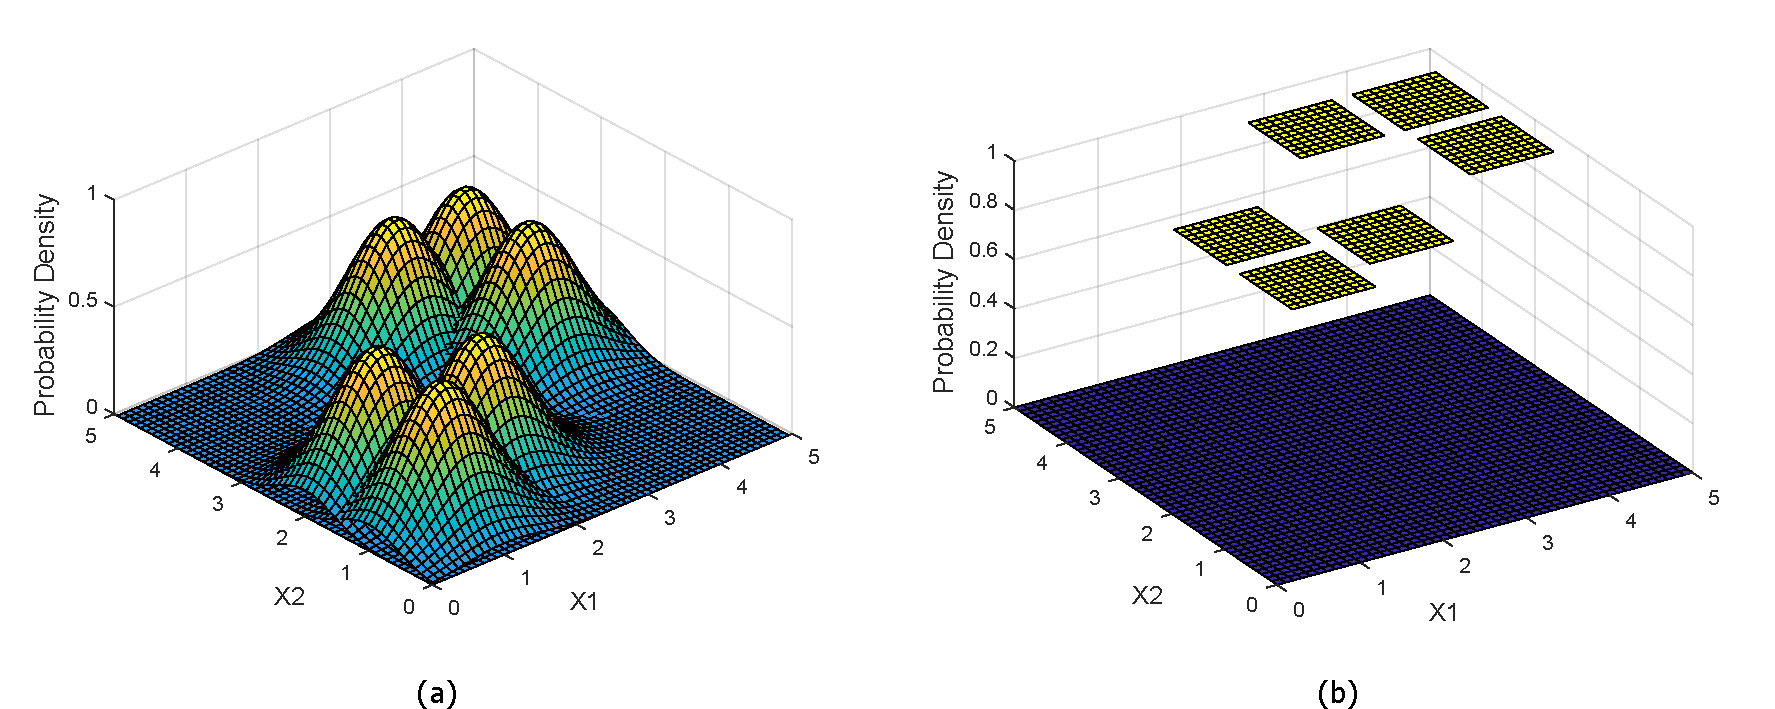
\includegraphics[height=0.4\columnwidth]{Figures/pdf.pdf}
   \label{fig:pdf}
   \caption{Approximation of probability density function}
\end{figure}


\end{enumerate}